\section{Environnement de programmation : CoDeSys}
    Dans ce module, nous programmerons sous l'environnement de développement CoDeSys. 
    \subsection{Présentation}
    CoDeSys est un environnement de développement intégré (IDE) permettant de programmer des automates programmables industriels (API). Il est basé sur la norme IEC 61131-3. Il permet de programmer des automates de différentes marques (Beckhoff, Wago, Schneider, \dots). Il est disponible sous Windows et sous Linux. Il est gratuit pour une utilisation non commerciale. 
    \subsection{Langages}
    CoDeSys permet de programmer des automates en utilisant les langages suivants : 
    \begin{itemize}
        \item Instruction List (IL).
        \item Ladder Diagram (LD).
        \item Function Block Diagram (FBD).
        \item Structured Text (ST).
        \item Sequential Function Chart (SFC).
    \end{itemize}
    \subsection{Architecture d'un programme}
    % Un programme CoDeSys est composé de plusieurs fichiers :
    % \begin{itemize}
    %     \item Un fichier de configuration du projet (.pro).
    %     \item Un fichier de configuration de l'automate (.hwf).
    %     \item Un fichier de configuration du réseau (.net).
    %     \item Un fichier de configuration de la communication (.opc).
    %     \item Un fichier de configuration de la visualisation (.visu).
    %     \item Un fichier de configuration de la cible (.xml).
    %     \item Un fichier de configuration de la bibliothèque (.lib).
    % \end{itemize}

    CoDeSys permet de programmer en Monotâche et en Multitâche :  
    \begin{itemize}
        \item 15 tâches périodiques au maximum.
        \item Priorité des taches de 1 à 15, de la plus prioritaire à la moins prioritaire.
        \item Temps de cycle compris entre \SI{100}{\micro\second} et \SI{10}{\second}.
    \end{itemize}

    \subsection{Unité de Programme -- Program Organisation Unit (POU)}
    Une unité de programme est un ensemble d'instructions qui peuvent être appelées depuis un autre programme. Il existe 3 types de POU :

    \begin{description}
        \item[Programme (Program -- PRG) : ] Un programme consiste en une série d'instruction pouvant produire une ou plusieurs valeurs en sortie. Il peut être appelé depuis un autre programme ou depuis un bloc fonction.
        Toutes les valeurs des variables du programme restent inchangées entre deux appels, quelque soit sa provenance. 
        
        \item[Bloc fonction (Function Block -- FB) : ] Un bloc fonction est un ensemble d'instructions pouvant produire une ou plusieurs valeurs en sortie. Il peut être appelé depuis un autre programme ou depuis un bloc fonction. Un bloc fonction sera toujours appelé au travers d'une instance de bloc fonction, copie du bloc fonction. Par conséquent, les valeurs des variables du bloc fonction seront inchangées entre deux appels d'une même instance uniquement. Ce type de POU sera particulièrement adapté à la programmation orientée objet que nous développerons dans ce module. 
        \item[Fonction (Function -- FUN) : ] Une fonction ne peut produire qu'une seule valeur en sortie. Elle peut être appelée par n'importe quel POU et les valeurs des variables ne persistent pas d'un appel à l'autre. 
    \end{description}


    \UPSTIinfo[Structure d'un POU]{
    Un POU est divisé en 2 parties :
    \begin{enumerate}
        \item Déclaration des variables.
        \begin{itemize}
            \item Variables d'entrées/sorties : \textbf{VAR\_INPUT}, \textbf{VAR\_OUTPUT}, \textbf{VAR\_IN\_OUT}.
            \item Variables Locales : \textbf{VAR}, \textbf{CONSTANT}.
        \end{itemize}
        \item Implémentation du POU
    \end{enumerate}
    %%% TODO: Ajouter un exemple de POU %%%
    }

    \UPSTIinfo[METHOD et ACTION]{
        Au sein d'une POU, il est possible de définir des méthodes et des actions. 
        \begin{description}
            \item[ACTION] : Portion de code toujours accessible qui ne peut utiliser que le \textbf{contexte} de l'entité à laquelle elle est associée. 
            \begin{description}
                \item[Exemple :] Une fonction RESET qui remet à zéro toutes les variables d'entrées/sorties d'un bloc fonction. 
            \end{description}
            \item[METHOD] :  Portion de code accessible qui utilise le contexte de l'entité à laquelle elle est associée, mais qui peut également créer son propre contexte. On peut définir \textbf{l'accessibilité} d'une méthode (PRIVATE, PROTECTED, PUBLIC, INTERNAL, \dots).
        \end{description}
    }

\subsection{Les types de données}
\subsubsection{Les types de données natifs}
CodeSys propose un ensemble de types de données natifs. Ces types de données sont définis par la norme IEC 61131-3. 
Pour chaque type de données, le tableau suivant précise son empreinte mémoire ainsi que les règles de nommage (préfixe) que nous utiliserons dans ce module. 


\begin{table}[htbp]
    \centering
    \begin{tabular}{|c|c|c|}
        \hline
        \rowcolor{gray!30} \textbf{Type de données} & \textbf{Empreinte mémoire} & \textbf{Règles de nommage} \\
        \hline
        BOOL & 1 bit & x \\
        \hline
        BYTE & 8 bits & by \\
        \hline
        SINT & 8 bits & si \\
        \hline
        USINT & 8 bits & usi \\
        \hline
        WORD & 16 bits & w \\
        \hline
        INT & 16 bits & i \\
        \hline
        UINT & 16 bits & ui \\
        \hline
        DWORD & 32 bits & dw \\
        \hline
        DINT & 32 bits & d \\
        \hline
        UDINT & 32 bits & udi \\
        \hline
        REAL & 32 bits & r \\
        \hline
        LWORD & 64 bits & lw \\
        \hline
        LINT & 64 bits & li \\
        \hline
        ULINT & 64 bits & uli \\
        \hline
        LREAL & 64 bits & lr \\
        \hline
        STRING & Variable & s \\
        \hline
    \end{tabular}
    \caption{Empreinte mémoire et règles de nommage des types de données natifs}
    \label{tab:types_donnees}
\end{table}

\subsubsection{Les types de données de datation}
\begin{table}[htbp]
    \centering
    \begin{tabular}{|c|c|c|}
        \hline
        \rowcolor{gray!30} \textbf{Type de données} & \textbf{Empreinte mémoire} & \textbf{Règles de nommage} \\
        \hline
        TIME (T\#) & 32 bits & tim \\
        \hline
        TIME\_OF\_DAY (TOD\#) & 32 bits & tod \\
        \hline
        DATE (D\#) & 32 bits & date \\
        \hline
        DATE\_AND\_TIME (DT\#) & 32 bits & dt \\
        \hline
    \end{tabular}
    \caption{Empreinte mémoire et règles de nommage des types de données de datation}
\end{table}

\subsubsection{Les tableaux}
Sous l'environnement CoDeSys, il est possible de déclarer des tableaux de variables. Ils peuvent être de dimension 1, 2 ou 3. Aussi, et contrairement au langage C, il est possible de définir le premier et le dernier indice. \textbf{Ainsi, le premier indice d'un tableau n'est pas forcément 0.} 

\UPSTIinfo[Déclaration d'un tableau]{La déclaration d'un tableau se fait à l'aide de la syntaxe suivante : \\~<nom> : ARRAY [<ll1>..<ul2>|,<ll2> <ul2>|,<ll3>..<ul3>] OF <type>;~. \\Avec ~<lli>~ la borne inférieure et ~<uli>~ la borne supérieure de la dimension i. }

Notre convention de nommage veut que l'on ajoute le prefix ~a<dim><type>~ à la déclaration d'un tableau. Avec ~<dim>~ le nombre de dimensions et ~<type>~ le préfixe correspondant à celui des éléments du tableau (Cf Table \ref{tab:types_donnees}).

Par exemple, pour définir un tableau ~tab~ de taille 10 de type ~WORD~ et un tableau ~tab2~ de taille 20x10 de type ~INT~, on écrira :
\begin{lstlisting}[language=ST]
VAR 
    a1wtab : ARRAY [0..9] OF WORD;
    a2itab2 : ARRAY [1..20, 1..10] OF INT;
END_VAR
\end{lstlisting}

Il est possible de récupérer le premier et le dernier indice d'un tableau à l'aide des fonctions ~LOWER_BOUND(<array_name>,<dim>)~ et ~UPPER_BOUND(<array_name>,<dim>)~, respectivement.

\UPSTIinfo[Tableau à longueur variable]{
    Lorsqu'un tableau est donné en ~VAR_IN_OUT~ d'une fonction, d'un bloc fonction ou d'une méthode, il est possible de ne pas préciser la taille du tableau par la syntaxe ~<nom> : ARRAY [*|, *|, *] OF <type>~. Dans ce cas, le tableau est dit à longueur variable. Il est possible de récupérer la taille du tableau à l'aide de la fonction ~SIZEOF(<array_name>)~.

    Par exemple, pour définir un tableau ~tab~ de dimension 1 et de taille variable de type ~WORD~, on écrira :\\~a1wtab : ARRAY [*] OF WORD;~
}

\subsubsection{Les structures}
\begin{UPSTIinfor}{Définition d'une structure}
    La définition d'une structure se fait à l'aide de la syntaxe suivante : 
    \begin{lstlisting}[language=ST]
TYPE <struct_name> :
    STRUCT
        <nom1> : <type1>;
        <nom2> : <type2>;
        ...
        <nomi> : <typei>;
    END_STRUCT
END_TYPE\end{lstlisting}

    Avec ~<nomi>~ le nom de la variable et ~<typei>~ le type de la variable. 
\end{UPSTIinfor}
Sous l'environnement CoDeSys, il est possible de déclarer des structures de variables. 
Notre convention de nommage veut que l'on ajoute le prefix ~T~ au nom d'une variable de type structure et ~m_<data_type><member_name>~ au nom d'un membre de la structure.

Par exemple, pour définir une structure ~TVerin~ contenant deux membres ~m_xSorti~ et ~m_xRENTRE~ de type ~BOOL~, on écrira : 
\begin{lstlisting}[language=ST]
TYPE TVerin :
    STRUCT
        m_xSorti : BOOL;
        m_xRENTRE : BOOL;
    END_STRUCT
END_TYPE\end{lstlisting}

Dans une structure uniquement, il est possible de déclarer des membres de type ~BIT~ afin de ne réserver qu'un seul bit mémoire (contrairement au type BOOL qui réserve 1 octet mémoire). Cela peut permettre d'assigner un nom à différents bits d'un registre, par exemple. 

\paragraph{Accès aux membres d'une structure : }
Il est possible d'accéder aux membres d'une structure à l'aide de la syntaxe ~<struct_name>.<member_name>~. Par exemple, pour accéder au membre ~m_xSorti~ de la structure ~enrVerin1~ de type ~TVerin~, on écrira ~enrVerin1.m_xSorti~.


\paragraph{Héritage : }
Le mot clé ~EXTENDS~ permet de définir une structure héritant d'une autre structure. La structure fille hérite de tous les membres de la structure mère auxquels elle peut ajouter ses propres membres. La syntaxe de cet héritage simple est alors : 

\begin{lstlisting}[language=ST]
TYPE <struct_fille> EXTENDS <struct_mere> :
    STRUCT
        <nom_n+1> : <type_n+1>;
        <nom_n+2> : <type_n+2>;
        ...
    END_STRUCT
END_TYPE\end{lstlisting}

\subsubsection{Les énumérations}
Une énumération est un type permettant de nommer des constantes entières. Elle augmente la lisibilité du code et permet de le rendre plus robuste. On peut par exemple définir une énumération ~ETAT~ contenant les constantes ~ETAT\_OUVERT~, ~ETAT\_FERME~, ~ETAT\_EN\_COURS~ et ~ETAT\_ERREUR~. Chaque ETAT correspond à une valeur entière que le développeur ne connait pas forcément. 

Par défaut, le premier élément de l'énumération vaut 0 et chaque élément suivant vaut l'élément précédent + 1. Il est possible de modifier cette valeur en utilisant l'opérateur ~|:=~. Par défaut, le type des valeurs de chaque élément est ~INT~. 

\begin{UPSTIinfor}{Définition d'une énumération}
    La définition d'une énumération se fait à l'aide de la syntaxe suivante : 
    \begin{lstlisting}[language=ST]
TYPE <enum_name> :
    (
        <nom1> |:= <valeur1>,
        <nom2> |:= <valeur2>,
        ...
        <nomi> |:= <valeuri>
    )|<base_data_type>|:= <valeur_par_defaut>;
END_TYPE\end{lstlisting}
\end{UPSTIinfor}

Par exemple, pour définir une énumération ~ETAT~ contenant les constantes ~ETAT\_OUVERT~, ~ETAT\_FERME~, ~ETAT\_EN\_COURS~ et ~ETAT\_ERREUR~, on écrira :
\begin{lstlisting}[language=ST]
TYPE ETAT :
    (
        ETAT_OUVERT,
        ETAT_FERME,
        ETAT_EN_COURS,
        ETAT_ERREUR
    ):= ETAT_OUVERT;
END_TYPE\end{lstlisting}

Voici alors un exemple de déclaration, d'initialisation et d'utilisation d'une variable de type ~ETAT~ :
\begin{lstlisting}[language=ST]
VAR
    etat : ETAT;
END_VAR
etat := ETAT_FERME;
IF etat = ETAT_FERME THEN
    (* Faire quelque chose *)
END_IF\end{lstlisting}

\UPSTIattention[Noms de constante identiques]{
    Si deux types énumération contiennent des constantes de même nom, il est alors impératif de préciser le type d'énumération. Par exemple, si on définit une énumération ~ETAT~ contenant les constantes ~ETAT\_OUVERT~, ~ETAT\_FERME~, ~ETAT\_EN\_COURS~ et ~ETAT\_ERREUR~ et une énumération ~ETAT\_VERIN~ contenant les constantes ~ETAT\_OUVERT~, ~ETAT\_FERME~, ~ETAT\_EN\_COURS~ et ~ETAT\_ERREUR~, il faudra alors écrire ~ETAT.ETAT\_OUVERT~ et ~ETAT\_VERIN.ETAT\_OUVERT~ pour différencier les deux constantes.
}

\subsubsection{Les unions}
Une union est un type permettant d'utiliser une même zone mémoire pour stocker des données de types différents. Cela signifie que la modification de la valeur d'une variable de l'union modifiera la valeur des autres variables.

Puisqu'il est partagé entre tous les membres de l'union, l'espace mémoire occupé par une union est égal à la taille de la variable occupant le plus d'espace mémoire.

\begin{UPSTIinfor}{Définition d'une union}
    La définition d'une union se fait à l'aide de la syntaxe suivante : 
    \begin{lstlisting}[language=ST]
TYPE <union_name> :
    UNION
        <nom1> : <type1>;
        <nom2> : <type2>;
        ...
        <nomi> : <typei>;
    END_UNION  
END_TYPE\end{lstlisting}
\end{UPSTIinfor}

Nos conventions de nommage veulent que l'on ajoute le prefix ~T~ au nom d'une variable de type union et ~m_<data_type><member_name>~ au nom d'un membre de l'union.

Enfin, des types de données spécifiques sont définis pour les unions : 
\begin{description}
    \item[ANY\_TYPE] : Type de données permettant de définir une union de type quelconque. Uniquement utilisable pour les interfaces
    \item[WSTRING] : Type de données permettant de définir une union de type chaine de caractères. Ce type de données est similaire au type STRING, mais l'encodage utilisé ici est UniCode au lieu de ASCII. 
\end{description}

\UPSTIremarque[Le type WSTRING]{
    Contrairement au STRING, le nombre de caractères affichable par une variable de type WSTRING d'une taille donnée dépend des caractères utilisés. En effet, certains caractères sont codés sur 1 octet, d'autres sur 2 octets. Par exemple, le caractère ~A~ est codé sur 1 octet, tandis que le caractère ~é~ est codé sur 2 octets. 
}

\subsubsection{Les pointeurs}
\UPSTIrappel[Pointeur]{
    Un pointeur est une variable contenant l'adresse mémoire d'une autre variable. Elle permet, de partager l'accès à une zone mémoire (variable) entre différents contextes. En langage C, par exemple, cela permet de créer des fonctions capables de modifier des variables locales à la fonction appelante. 

    Lorsque vous avez utilisé la fonction \lstinline[language=c]{scanf}, vous avez passé en paramètre l'adresse de la variable à modifier à l'aide de l'opérateur \lstinline[language=c]{\&}. Cela permet à la fonction \lstinline[language=c]{scanf} de modifier la valeur de la variable passée en paramètre.
}

\begin{UPSTIinfor}{Définition d'un pointeur}
    La définition d'un pointeur se fait à l'aide de la syntaxe suivante : 
    \begin{lstlisting}[language=ST]
<pointer_name> : POINTER TO <type>;\end{lstlisting}

Ici, ~<type>~ peut désigner le type d'une variable, une fonction, un bloc fonction, une méthode ou même un POU. 
\end{UPSTIinfor}

Les opérateurs disponibles pour l'utilisation de pointeurs sont les suivants : 
\begin{itemize}
    \item ~^~ : Opérateur de déréférencement. Il permet d'accéder à la valeur pointée par le pointeur. 
    \item ~ADR~ : Opérateur d'adressage. Il permet d'accéder à l'adresse mémoire pointée par le pointeur.
    \item ~[ ]~ : Opérateur d'indexation : Il permet d'accéder à un élément d'un tableau pointé par un pointeur.
\end{itemize}

Nos rêgles de nommage veulent que l'on ajoute le prefix ~p~ au nom d'une variable de type pointeur.

\UPSTIexemple{
    \begin{minipage}[t]{0.45\linewidth}
    \begin{lstlisting}[language=ST]
VAR
    piA : POINTER TO INT := 0;
    iAlpha AT %MW1: INT := 7;
    iBeta AT %MW3: INT := 4;
    piB : POINTER TO INT := ADR(iBeta);
    dwGapInBytes: DWORD; (* en octet *)
END_VAR\end{lstlisting}
    \end{minipage}
    \hfill
    \begin{minipage}[t]{0.45\linewidth}
\begin{lstlisting}[language=ST]
(* Traitement *)
piA := ADR (iAlpha);
piA^ := 0 ; (* <=> iAlpha := 0; *)
piB[0] := 0 ; (* <=> iBeta := 0; *)
dwGapInBytes := piB - piA; (* = 4 *)\end{lstlisting}
    \end{minipage}
}

\subsubsection{Les références}
Sous CodeSys, une référence possède des propriétés similaires à celles d'un pointeur. Elle présente des avantages et inconvénients suivants par rapport à un pointeur :
\begin{minipage} [t]{0.45\linewidth}
    \begin{itemize}
        \item Plus simple à utiliser : pas besoin d'utiliser l'opérateur ~^~ pour accéder à la valeur pointée.
        \item Syntaxe plus simple
        \item Sécurisée sur le type : le compilateur vérifie que la référence pointe bien sur une variable du type attendu.
    \end{itemize}
    
\end{minipage}\hfill
\begin{minipage} [t]{0.45\linewidth}
    \begin{itemize}
        \item Il est impossible de modifier la variable pointée par la référence,
        \item On ne peut référencer que des variables (pas de fonctions, blocs fonction, méthodes ou POU).
    \end{itemize}
\end{minipage}

La fonction ~__ISVALIDREF(ref_int~ permet de vérifier si une référence est valide ou non. Elle renverra ~TRUE~ si la référence est valide (pointe vers une variable et non 0), ~FALSE~ sinon.

\UPSTIexemple{
    \begin{minipage}[t]{0.45\linewidth}
    \begin{lstlisting}[language=ST]
VAR
    ref_int: REFERENCE TO INT := 0;
    iAlpha: INT := 7;
    iBeta: INT := 4;
    xRef: BOOL;
END_VAR\end{lstlisting}
    \end{minipage}
    \hfill
    \begin{minipage}[t]{0.45\linewidth}
\begin{lstlisting}[language=ST]
(* Traitement *)
xRef := __ISVALIDREF (ref_int); (* FALSE *)
ref_int REF := iAlpha ; (*<=> ADR (iAlpha); *)
xRef := __ISVALIDREF (ref_int) ; (* TRUE *)
ref_int := 0 ; (*<=> ADR(iAlpha)^:= 0 ; *);
ref_int REF := iBeta (*<=> ADR (iBeta)*);
ref_int := 0 ; (* <=> iBeta := 0 ; *)
\end{lstlisting}
    \end{minipage}
}
\subsection{Le langage SFC}
Le langage SFC (\textit{Sequential Function Chart}) est un langage graphique permettant de décrire le comportement d'un système automatisé. Il est basé sur le formalisme des GRAFCET (\textit{GRAphe Fonctionnel de Commande Etape Transition}).

\UPSTIremarque{Bien qu'ils soient très similaires à première vue, le GRAFCET est un langage  destiné à la spécification alors que le SFC est un langage destiné à la programmation.}

\begin{UPSTIinfor}{Rappels sur le SFC}
Un graph SFC consiste en une succession d'\textbf{étapes} et de \textbf{transitions}. A l'origine, une seule étape initiale est active. A chaque cycle, les transitions sont évaluées. Une transition est dite \textbf{franchissable} si sa \textbf{réceptivité} est ~TRUE~ et que l'étape qui la précède est active.
Si une transition est franchissable, elle est franchie et l'étape suivante devient active.
Lorsqu'une étape est active, elle exécute l'ensemble des \textbf{actions} qui lui sont associées.

Rappel de vocabulaire : 
\begin{description}
    \item[Étape] : Une étape est un ensemble d'actions qui s'exécutent en parallèle. Une étape est représentée par un rectangle. 
    \item[Transition] : Une transition est un ensemble de conditions qui doivent être vérifiées pour passer d'une étape à une autre. Une transition est représentée par un trait horizontal. 
    \item[Action] : Une action est une opération élémentaire qui peut être réalisée par le système. Une action est représentée par un rectangle vertical.
    \item[Réceptivité] : Une réceptivité est une condition booléenne qui doit être vérifiée pour qu'une transition soit franchissable.
\end{description}
\end{UPSTIinfor}

\subsubsection{Les actions en SFC}

\begin{wrapfigure}{r}{0.3\linewidth}
    \centering
    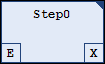
\includegraphics[width=.5\linewidth]{_cds_sfc_step_active.png}
    \caption{Action en SFC}
    \label{fig:ActionSFC}
\end{wrapfigure}
Sous CodeSys, l'activation d'une étape entraîne l'exécution de l'ensemble des actions qui lui sont associées. Elles peuvent être exécutées : 

\begin{enumerate}
    \item Une seule fois à l'activation de l'étape (Les \textbf{Actions d'entrées} -- \textbf{Entry actions}).
    \begin{itemize}
        \item La présence d'une action d'entrée est indiquée par un E dans le coin inférieur gauche de l'étape.
    \end{itemize}
    \item Exécutée à chaque cycle tant que l'étape est active (Les \textbf{Actions actives} -- \textbf{actions}).
    \begin{itemize}
        \item La présence d'une action active est indiquée par un triangle dans le coin supérieur droit de l'étape.
    \end{itemize}
    \item Une seule fois à la désactivation de l'étape (Les \textbf{Actions de sortie} -- \textbf{Exit actions}).
    \begin{itemize}
        \item La présence d'une action de sortie est indiquée par un X dans le coin inférieur droit de l'étape.
    \end{itemize}
\end{enumerate}

A chaque action est associée un qualificatif dont la signification est donnée dans le tableau suivant : 

\begin{center}
    

\begin{tabular}[t]{l|l|p{0.5\linewidth}}
   \textbf{Qualificatif} & \textbf{Nom} & \textbf{Description} \\
    \hline
    N & Non-stored & L'action est exécutée tant que l'étape est active\\\hline
    S0 & Stored & L'action est exécutée dès que l'étape est active. Elle restera active jusqu'à ce qu'elle soit désactivée (même après que l'étape n'est plus active)\\\hline
    R0 & Reset & L'action est désactivée et cesse donc d'être exécutée\\\hline
    L & time Limited & L'action commence son exécution à l'activation de l'étape et s'arrête après un temps défini ou lorsque l'étape est désactivée\\\hline
    D & time Delayed & L'action commence son exécution après un temps défini suivi l'activation de l'étape et s'arrête lorsque l'étape est désactivée\\\hline
   P & Pulse & L'action est exécutée une seule fois à l'activation de l'étape\\\hline
   SD & Stored and time Delayed & L'action commence son exécution après un temps défini suivi l'activation de l'étape, même si cette dernière n'est plus active. L'action s'exécute tant qu'elle n'est pas désactivée (même après que l'étape n'est plus active)\\ \hline
   DS & Delayed and Stored & L'action commence son exécution après un temps défini suivi l'activation de l'étape, si celle-ci est toujours active. L'action s'exécute tant qu'elle n'est pas désactivée (même après que l'étape n'est plus active)\\ \hline
   SL & Stored and time Limited & L'action commence son exécution à l'activation de l'étape et s'arrête après un temps défini ou lorsque l'étape est désactivée. \\
   \hline
\end{tabular}
\end{center}

\subsubsection{Les transitions en SFC}
La réceptivité associée à une transition sous CodeSys peut être vue comme l'appel d'une fonction. En effet, il est possible d'exécuter un algorithme pour évaluer la réceptivité d'une transition.


\subsubsection{Les drapeaux d'un graph SFC}
Les drapeaux sont des variables qui (souvent booléennes) qui permettent le contrôle et le suivi de l'évolution d'un graph SFC. 
Le tableau suivant décrit les principaux drapeaux que nous rencontrerons : 
\begin{center}
    \begin{tabular}[t]{l|p{0.6\linewidth}}
        \hline
        ~SFCInit : BOOL~ & Son passage à ~TRUE~ entraine l'initialisation normalisée du graph SFC et de tous les drapeaux. Tant qu'elle est à ~TRUE~, le graph SFC reste dans son état initial, sans qu'aucune action ne soit exécutée.\\\hline
        ~SFCReset : BOOL~ & Son passage à ~TRUE~ entraine la réinitialisation du graph SFC et de tous les drapeaux. Tant qu'elle est à ~TRUE~, le graph SFC reste dans son état initial et \textbf{l'action associée à l'étape initiale est exécutée}.\\\hline
        ~SFCPause : BOOL~ & Son passage à ~TRUE~ entraine la mise en pause du graph SFC. \\\hline    
        ~SFCTrans : BOOL~ & Passe à ~TRUE~ à chaque franchissement d'une transition. \\\hline
        ~SFCCurrentStep : STRING~ & Contient le nom de l'étape active. Si plusieurs étapes sont active, celui de l'étape la plus à droite. \\\hline
    \end{tabular}
\end{center}

%%% TODO : Notion de grafcet partiel coopérant %%%


\section{Programmation classique hiérarchisée à l'aide du GMMA}
Cette section propose un paradigme de programmation d'une application automatisée à l'aide du GMMA sur l'application e!Cockpit.

L'application consiste en une tâche principale nommée \emph{MainTask} qui est exécutée périodiquement. Cette tâche appelle une seule unité de programme (POU) : \emph{MainProgram} qui mettra en oeuvre un GMMA en langage SFC. Chaque étape du GMMA sera associée à une POU correspondant au mode à jouer. Enfin, la POU de chaque mode sera implémentée dans un langage adapté au type de tâche à réaliser. Enfin, on ajoute deux gestionnaires d'événements : \emph{}

Ce paradigme permet de respecter une hiérarchisation des tâches et des POUs : Le GMMA est préemptif et autorise ou non les différents modes en fonction de l'état du système.

\paragraph{La tâche principale} fonctionne avec une priorité comprise entre 4 et 15. Elle est exécutée cycliquement avec une période qui doit être compatible avec la dynamique du procédé. Une surveillance doit être mise en place par l'intermédiaire d'un watchdog (chien de garde) réglé avec une sensibilité de 1.
Cette tâche appelle alors une seule POU : le programme principal \emph{MainProgram}.

\begin{UPSTIinfor}{Dynamique du procédé}
    La dynamique du procédé correspond à la vitesse à laquelle le procédé peut évoluer. Afin de fonctionner correctement, le système automatisé doit être capable de réagir à tous les événements du procédé. Pour cela, la période de la tâche principale doit être inférieure à cette dynamique.

    Pour déterminer ce temps, on peut effectuer une étude s'intéressant à l'entrée la plus rapide qui doit être prise en compte par le système automatisé. Le cycle de l'automate doit alors être plus rapide que le temps de cette entrée.

    Par exemple, si le système automatisé doit réagir à une entrée TOR, il faut déterminer le temps de changement d'état de cette entrée et s'assurer que le cycle de l'automate est plus rapide que ce temps en configurant le watchdog.
\end{UPSTIinfor}

\paragraph{La POU MainProgram}, appelée par la tâche principale, gère la POU associée au GMMA. Cela signifie qu'elle appellera la POU du GMMA après avoir effectué les vérifications nécessaires. Par exemple, elle pourra faire un reset du GMMA au premier cycle de l'automate.

\paragraph{La POU du GMMA} est une POU de type SFC. Elle est composée de plusieurs étapes. Chaque étape est associée à une POU correspondant à un mode de fonctionnement.
A chaque étape, on utilise les actions d'entrée pour paramétrer le mode puis l'action active pour que la POU correspondante soit appelée à chaque cycle automate.

\paragraph{Les POU des modes} sont des POUs implémentées en ST ou en SFC. Elles sont appelées par la POU du GMMA et sont exécutées à chaque cycle automate si le mode correspondant est actif.

\paragraph{Les gestionnaires d'événements} sont des POUs implémentés en ST ou en SFC.  Ils permettent de gérer les événements qui ne sont pas liés à un mode de fonctionnement. Typiquement, on définira un événement pour le premier cycle (\emph{OnFirstRun}) pour effectuer diverses initialisations (par exemple un booléen global \emph{xFirstCycleRun} qui fera un reset du GMMA) et un événement en fin de cycle (\emph{OnPrepareStop}) qui pourra fixer les modes de repli si nécessaire. On peut aussi utiliser, par exemple, un gestionnaire d'événement pour gérer les alarmes.

\paragraph{Exemple}
Cette section présente un code d'exemple d'application du GMMA dans une structure hiérarchisée.
\paragraph{Variable globales (Global Variable List -- GVL)} :
On définit une variable globale indiquant que l'on se trouve dans le premier cycle :
\begin{lstlisting}[language=ST]
VAR_GLOBAL
    xFirstCycleRun : BOOL;
END_VAR
\end{lstlisting}

\paragraph{2 Events Handlers :}
On écrit une fonction pour le premier cycle :
\begin{lstlisting}[language=ST]
FUNCTION OnFirstRun : DWORD
    VAR_IN_OUT
        EventPrm : CmpApp.EVTPARAM_CmpApp;
    END_VAR

    GVL.xFirstCycleRun := TRUE;
    OnFirstRun := 0;\end{lstlisting}

\paragraph{Tâche principale}
La tâche principale est configurée avec une période de \SI{40}{\milli\second} et une priorité de 4. Elle appelle la POU \emph{MainProgram}. Le watchdog est configuré avec une sensibilité de 1 et un temps de \SI{60}{\milli\second}.

\paragraph{Le programme principal (MainProgram) :}
Le programme principal, en langage ST, s'occupe de lancer correctement le GMMA :
\begin{lstlisting}[language=ST]
PROGRAM MainProgram
    VAR
        xSFRResetGmma : BOOL := FALSE;
    END_VAR

    IF GVL.xFirstCycleRun THEN
        xSFRResetGmma := TRUE;
        GVL.xFirstCycleRun := FALSE;
    END_IF

    GM_Gmma(SFRRESET := xSFRResetGmma);\end{lstlisting}

\paragraph{Le GMMA :}
Le GMMA est implémenté en langage SFC. La déclaration des variables est la suivante :
\begin{lstlisting}[language=ST]
PROGRAM GM_Gmma
    VAR_IN_OUT 
        SFRReset : BOOL;
    END_VAR
    
    VAR
        xD1Reset : BOOL := FALSE;
        xF1A2Reset : BOOL := FALSE;
    END_VAR\end{lstlisting}


\lstDeleteShortInline~
\pagebreak
\begin{UPSTIactivite}[][Application : Etape D1 du GMMA]
    \UPSTIquestion{Dessiner la première étape du GMMA, appelée GM\_S\_D1 associée à sa transition.}
    \UPSTIquestion{Écrire l'action d'entrée \lstinline{GM_Gmma.GM_AP1_ResetChartD1} qui met à \lstinline{TRUE} le booléen \lstinline{xD1Reset}.}
    \UPSTIquestion{Écrire l'action active \lstinline{GM_Gmma.GM_AN_D1_ArretUrgence} qui :}
    \begin{itemize}
        \item Passe à \lstinline{TRUE} le booléen \lstinline{xD1Reset} si nécessaire.
        \item Appelle la POU \lstinline{D1_ArretUrgence} avec le paramètre \lstinline{SFCReset}
        \item Appelle la POU \lstinline{D1_ArretUrgencePost} pour le traitement post arrêt d'urgence.
    \end{itemize}
    \vspace{15cm}
\end{UPSTIactivite}

\paragraph{Les POU spécifiques à chaque mode} sont implémentées en langage ST, LADDER ou SFC selon si le comportement associé est combinatoire ou séquentiel.

Par exemple, la POU \lstinline{D1_ArretUrgence} implémenté en SFC aura les déclarations suivantes :

\begin{lstlisting}
PROGRAM D1_ArretUrgence
    VAR_IN_OUT
        SFCReset : BOOL;
    END_VAR\end{lstlisting}



